\begin{frame}{Origins of Molecular Dynamics (MD)}
    \begin{itemize}
        \item Modern MD was developed in the 1950s, influenced by Monte Carlo methods popularized at Los Alamos National Laboratory.
        \pause
        \bigskip
        \item However, interest in the evolution of N-body systems dates back to the 17th century with Isaac Newton, focusing mainly on celestial mechanics.
        \pause
        \bigskip
        \item Many key numerical algorithms were created before computers. For example, the \textbf{Verlet integration algorithm}, the most common today, was used as early as 1791 by Jean Baptiste Joseph Delambre.
    \end{itemize}
\end{frame}

%------------------------------------------------

\begin{frame}{Pre-Computational Methods}
    Before digital computers, modeling was done in other ways:
    \pause
    
    \begin{itemize}
        \item \textbf{Analog computers} were used to integrate the equations of motion.
        \pause
        \item Some scientists built \textbf{physical models} with spheres to replicate the structure of liquids and study their behavior.
    \end{itemize}
    \pause
    
    \begin{block}<4->{The Fermi-Pasta-Ulam-Tsingou Problem}
        To understand the origin of irreversibility, Enrico Fermi and his collaborators used the \textbf{MANIAC I} computer in 1953 to simulate the time evolution of a many-body system.
    \end{block}
\end{frame}

%------------------------------------------------

\begin{frame}{FPU Problem Graph}
    \begin{figure}
        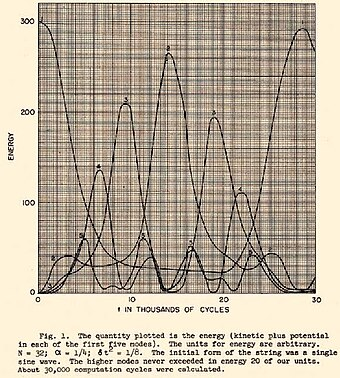
\includegraphics[width=0.5\textwidth]{images/MANIAC.png}
        \caption{Energy vs. time for one of the first N-body systems simulated by Fermi, showing unexpected and non-irreversible behavior.}
    \end{figure}
\end{frame}

%------------------------------------------------

\begin{frame}{Towards Realistic Matter Simulations}
    \footnotesize
    With the advent of more powerful computers, simulations became more realistic:
    \pause
    
    \begin{itemize}
        \item \textbf{1957:} Alder and Wainwright simulated elastic collisions between hard spheres using an IBM 704 computer.
        \pause
        \bigskip
        \item \textbf{1960:} Gibson and his team performed perhaps the first realistic simulation, modeling radiation damage in solid copper.
        \pause
        \bigskip
        \item \textbf{1964:} Rahman simulated liquid argon using a \textbf{Lennard-Jones potential}, with results that agreed well with experimental data.
    \end{itemize}
    \pause
    
    \begin{alertblock}<4->{The Legacy of the Lennard-Jones Potential}
        Today, it remains one of the most widely used potentials for describing simple substances and as a component of more complex force fields.
    \end{alertblock}
\end{frame}

%------------------------------------------------

\begin{frame}{The Molecular Dynamics Algorithm: Key Steps}
    \begin{block}{Algorithm Steps}
        \begin{enumerate}
            \item \textbf{Initialization:} Initial positions and velocities are assigned to the atoms.
            \pause
            \item \textbf{Force Calculation:} The forces on each atom are calculated, either from classical ($F = -\nabla V(\vec{r})$) or quantum ($F = F(\Psi(\vec{r}))$) potentials.
            \pause
            \item \textbf{Integration:} Positions and velocities are updated for a small time step ($\Delta t$) using an integrator.
            \pause
            \item \textbf{Iteration:} Steps 2 and 3 are repeated for the time required to observe the system's evolution.
        \end{enumerate}
    \end{block}
\end{frame}

%------------------------------------------------

\begin{frame}{MD Algorithm Graph}
    \begin{figure}
        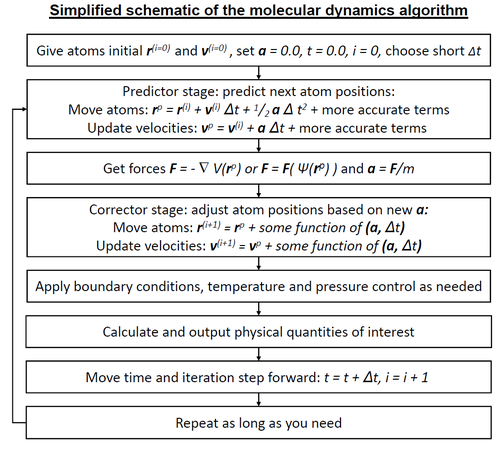
\includegraphics[width=0.5\textwidth]{images/algorithm.png}
        \caption{Simplified schematic of the Molecular Dynamics algorithm.}
    \end{figure}
\end{frame}